\documentclass{article}
\usepackage[utf8]{inputenc}
\usepackage[english]{babel}
\usepackage[]{amsthm}
\usepackage[]{amssymb}
\usepackage{amsmath}
\usepackage{gensymb}
\usepackage{blindtext}
\usepackage{geometry}
 \geometry{
 a4paper,
 total={170mm,257mm},
 left=20mm,
 top=20mm,
 }
\usepackage{pgfplots}

\pgfplotsset{width=7cm,compat=1.9}

% We will externalize the figures
\usepgfplotslibrary{external}
\tikzexternalize

\newcommand{\ihat}{\;\hat{\textbf{\i}}}
\newcommand{\jhat}{\;\hat{\textbf{\j}}}
\newcommand{\khat}{\;\hat{\textbf{k}}}
\newcommand{\rvec}{\vec{r}(t)}
\newcommand{\drvec}{\vec{r}\;'(t)}
\newcommand\vv[1]{\langle #1 \rangle}
\newcommand\vc[2]{\vec{#1}(#2)}
\newcommand\vcd[2]{\vec{#1}\;'(#2)}
\newcommand\vcdd[2]{\vec{#1}\;''(#2)}
\newcommand\vcddd[2]{\vec{#1}\;'''(#2)}
\newcommand\mgv[1]{\|#1\|}
\newcommand\mgvv[2]{\sqrt{\left(#1\right)^2 + \left(#2\right)^2}}
\newcommand\mgvvv[3]{\sqrt{\left(#1\right)^2 + \left(#2\right)^2 + \left(#3\right)^2}}
\newcommand\rr{\quad\Rightarrow\quad}


\title{Chapter 13 Section 3 \& 4 Problem Set}
\author{Andry Paez}

\begin{document}
\maketitle
\section*{Section 3: Arc Length and Curvature}

\subsection*{Problem 1a}

Use Equation 2 to compute the length of the given line segment.

\[
    \vec{r}(t)  = \langle{3-t, 2t, 4t + 1}\rangle \quad 1 \leq{t} \leq{3}
\]

\subsection*{Solution}

Let the length of the line segment be 

\begin{align*}
    L = \int_{a}^{b} \sqrt{(\frac{dx}{dt})^2 + (\frac{dy}{dt})^2 + (\frac{dz}{dt})^2} \;dt 
    \Rightarrow L = \int_{a}^{b} \|\vec{r}\;'(t)\| \;dt
\end{align*}

\[
    D: \{\:t \;|\; 1 \leq t \leq 3\:\}
\]

\begin{align*}
    \vec{r}\:'(t)  = \langle{-1, 2, 4}\rangle \Rightarrow
    L &= \int_{1}^{3} \sqrt{(-1)^2 + (2)^2 + (4)^2} dt
      &= \int_{1}^{3} \sqrt{21} dt &= \sqrt{21}t \; \Big|_{1}^{3} = \sqrt{21}(3) - \sqrt{21}(1) = 2\sqrt{21}
\end{align*}

   
\subsection*{Problems 3-7 odd}

Find the length of the curve.

\subsubsection*{3. $\vec{r}\;(t) = \langle{t, 3\cos{t}, 3\sin{t}} \rangle \quad 25 \leq t \leq 5$}
\subsubsection*{Solution}

\begin{align*}
    \vec{r}\;'(t) = \langle{1, -3\sin{t}, 3\cos{t}} \rangle \Rightarrow
    L &= \int_{-5}^{5} \sqrt{1^2 + (-3\sin{t})^2 + (3\cos t)^2}\;dt \\
    &= \int_{-5}^{5} \sqrt{1 + 9\sin^2t + 9\cos^2t}\; dt\\ 
    &= \int_{-5}^{5} \sqrt{1 + 9(1)}\; dt \\
    &= \int_{-5}^{5} \sqrt{10}\; dt \\ 
    &= \sqrt{10}t\; \Big|_{-5}^{5} dt = \sqrt{10}(5) - \sqrt{10}(-5) = 10\sqrt{10}
\end{align*}


\[
\]

\subsubsection*{5. $\vec{r}\;(t) = \langle{\sqrt{2}t, e^{t}, e^{-t}} \rangle \quad 0 \leq t \leq 1$}
\subsubsection*{Solution}

\begin{align*}
    \vec{r}\; '(t) = \langle{\sqrt{2}, e^{t}, -e^{-t}} \rangle \Rightarrow
    L &= \int_{0}^{1} \sqrt{(\sqrt{2})^2 + (e^{t})^{2} + (-e^{-t})^{2}}\; dt \\
      &= \int_{0}^{1} \sqrt{2 + e^{2t} + e^{-2t}}\; dt \\ 
      &= \int_{0}^{1} \sqrt{(e^{t} + e^{-t})^2}\; dt \\
      &= \int_{0}^{1} e^{t} + e^{-t}\; dt \\
      &= e^{t} - e^{-t}\; \Big|_{0}^{1} = (e^{1} - \frac{1}{e^1}) - (e^{0} - \frac{1}{e^0}) = e - \frac{1}{e} - 1 + 1 = e - \frac{1}{e}
\end{align*}



\subsubsection*{7. $\vec{r}\;(t) = \langle{1, t^2, t^3} \rangle \quad 0 \leq t \leq 1$}
\subsubsection*{Solution}

\begin{align*}
    \vec{r}\; '(t) = \langle{0, 2t, 3t^2} \rangle \Rightarrow
    L &= \int_{0}^{1} \sqrt{(0)^2 + (2t)^2 + (3t^2)^2}\; dt \\
      &= \int_{0}^{1} \sqrt{4t^2 + 9t^4}\; dt \\
      &= \int_{0}^{1} \sqrt{t^2(4 + 9t^2)}\; dt \\
      &= \int_{0}^{1} t\sqrt{4 + 9t^2}\; dt \\
\end{align*}
Using u-substitution,
\begin{align*}
    u^2 &= 4 + 9t^2 \\
    2udu &= 18t\; dt \\
    \frac{u\;du}{9} &= t\; dt \\
    \int_{0}^{1} t\sqrt{4 + 9t^2}\; dt
                    &= \int_{0}^{1} u \cdot(\frac{1}{9} u) \; du
                    &= \frac{1}{9} \int_{0}^{1} u^2\; du
                    &= \frac{1}{9} (\frac{1}{3} u^3) \Big|_{2}^{\sqrt{13}}
                    &= \frac{1}{27} (u^3) \Big|_{2}^{\sqrt{13}}
                    &= \frac{1}{27} (13^{\frac{3}{2}} - 2^3) = \frac{13\sqrt{13}}{27} - 3
\end{align*}

\subsection*{Problems 19-23 odd}

(a) Find the unit tangent and unit normal vectors $\vec{T}(t)$ and $\vec{N}(t)$. \\
(b) Use Formula 9 to find the curvature.


\subsubsection*{19. $\vec{r}(t) = \langle{t^2,\; \sin{t} - t\cos{t},\; \cos{t} + t\sin{t}} \rangle, \quad t > 0$}
\subsubsection*{Solution}
a. 
\[
    \vec{T}(t) = \frac{\drvec}{\|\drvec\|}   
\]
\begin{align*}
    \drvec &= \langle 2t, \cos t - \cos t + t\sin t, -\sin t + \sin t + t\cos t \rangle = \langle 2t, t\sin t, t\cos t \rangle \\
    \|\drvec\| &= \sqrt{4t^2 + t^2\sin^2t + t^2\cos^2t} = \sqrt{4t^2 + t^2} = \sqrt{5t^2} = \sqrt{5}t \quad [\cos^2t + \sin^2t = 1] \\ 
    \vec{T}(t) &= \frac{\langle 2t, t\sin t, t\cos t \rangle}{\sqrt{5}t} = \frac{1}{\sqrt{5}}\langle 2, \sin t, \cos t \rangle
\end{align*}
\[
    \vec{N}(t) = \frac{\vec{T}\;'(t)}{\|\vec{T}\;'(t)\|}
\]
\begin{align*}
    \vec{T}\;'(t) &= \frac{1}{\sqrt{5}}\langle 0, \cos t, -\sin t \rangle \\
    \|\vec{T}\;'(t)\| &= \frac {1}{\sqrt 5} \sqrt{0^2 + \cos^2t + \sin^2t} = \sqrt{1} = \frac{1}{\sqrt 5} \\
    \vec{N}(t) &= \frac{ \frac{1}{\sqrt{5}} \langle 0, \cos t, -\sin t \rangle}{\frac{1}{\sqrt{5}}} = \langle 0, \cos t, -\sin t \rangle 
\end{align*}
b. 
\begin{align*}
    \kappa(t) &= \frac{\|\vec{T}\;'(t)\|}{\|\drvec\|} = \frac{\frac{1}{\sqrt 5}}{\sqrt 5t} = \frac{1}{5t}
\end{align*}

\subsubsection*{21. $\vec{r}(t) = \langle{t, t^2, 4} \rangle$}

\subsubsection*{Solution}
a. 
\begin{align*}
    \drvec &=  \ihat +  2t\jhat \\ 
    \|\drvec\| &= \sqrt{1^2 + (2t)^2} = \sqrt{1 + 4t^2}  \\
    \vec T (t) &=  \frac{\ihat + 2t\jhat}{\sqrt{1 + 4t^2}} = \frac{1}{\sqrt{1 + 4t^2}}(\ihat + 2t\jhat) \\
    \frac{d}{dt} &= [f(t)\vec u (t)] = f'(t)\vec u (t) + f(t)\vec u \;'(t) \quad [vector\;product\;rule] \\  
    \vec T \;'(t) &= -\frac{4t}{(1+4t^2)^{\frac 3 2}}(\ihat + 2t\jhat) + \frac{1}{(1 + 4t^2)^{\frac 1 2}}(2\jhat) \\
                  &= \frac{1}{(1 + 4t^2)^{\frac 3 2}}\left(-4t(\ihat + 2t\jhat) + (1+4t^2)(2\jhat)\right) = \frac{1}{(1 + 4t^2)^{\frac 3 2}}(-4t\ihat - 8t^2\jhat + 2\jhat + 8t^2\jhat) \\
                  &= \frac{1}{(1 + 4t^2)^{\frac 3 2}}(-4t\ihat + 2\jhat) \\
    \| \vec T \;'(t)\| &= \frac{1}{\left(1+4t^2\right)^{\frac 3 2}}\sqrt{(-4t)^2 + 2^2} = \frac{1}{(1 + 4t^2)^{\frac 3 2}} \sqrt{16t^2 + 4} = \frac{1}{(1 + 4t^2)^{\frac 3 2}}\sqrt{4(4t^2 + 1)} = \frac{2}{(1 + 4t^2)^{\frac 3 2}}\sqrt{1+4t^2} \\
                       &= \frac{2}{1+4t^2} \\
    \vec N (t) &=  \frac{\vec T\;'(t)}{\|\vec T\;'(t)\|} = \frac{1}{(1+4t^2)^{\frac 3 2}}(-4t\ihat + 2\jhat) \; \cdot \; \frac{1+4t^2}{2} = \frac{(1+4t^2)^1}{2(1+4t^2)^{\frac 3 2}}(-4t\ihat + 2\jhat) = \frac{1}{\sqrt{1+4t^2}}(-2t\ihat + \jhat)
\end{align*}
b.
\begin{align*}
    \kappa (t) = \frac{\|\vec T\;'(t)\|}{\|\drvec\|} = \frac{2}{1+4t^2} \;\cdot\; \frac{1}{(1+4t^2)^\frac 1 2} = \frac{2}{(1+4t^2)^{\frac 3 2}}
\end{align*}
\subsubsection*{23. $\vec{r}(t) = \langle{t, \frac{1}{2}t^2, t^2} \rangle$}
\subsubsection*{Solution}
a. 
\begin{align*}
    \drvec &= \langle 1, t, 2t \rangle \\
    \|\drvec\| &= \sqrt{1^2 + t^2 + (2t)^2} = \sqrt{1 + 5t^2} \\ 
    \vec T(t) &= \frac{\drvec}{\|\drvec\|} = \frac{\langle 1, t, 2t \rangle}{\sqrt{1 + t^2 + 4t^2}} = \frac{1}{\sqrt{1 + 5t^2}}\langle 1, t, 2t \rangle \\
    \frac{d}{dt} &= [f(t)\vec u (t)] = f'(t)\vec u (t) + f(t)\vec u \;'(t) \quad [vector\;product\;rule] \\  
    \vec T\;'(t) &= -\frac{5t}{(1+5t^2)^{\frac 3 2}}\langle 1, t, 2t\rangle + \frac{1}{(1+5t^2)^\frac 1 2}\langle 0, 1, 2 \rangle \\
                 &= \frac{1}{(1+5t^2)^{\frac 3 2}}\left(-5t \langle 1, t, 2t \rangle + (1+5t^2)\langle 0, 1, 2 \rangle\right) \\
                 &= \frac{1}{(1+5t^2)^{\frac 3 2}}\left(\langle -5t, -5t^2, -10t^2 \rangle + \langle 0, 1+5t^2, 2+10t^2 \rangle\right) = \frac{1}{(1+5t^2)^{\frac 3 2}} \langle -5t, 1, 2 \rangle \\
    \|\vec T\;'(t)\| &= \frac{1}{(1+5t^2)^{\frac 3 2}}\sqrt{(-5t)^2 + 1^2 + 2^2} = \frac{1}{(1+5t^2)^{\frac 3 2}}\sqrt{25t^2 + 5} = \frac{1}{(1+5t^2)^{\frac 3 2}}\sqrt{5(5t^2 + 1)} \\
                     &= \frac{\sqrt 5 (1+5t^2)^{\frac 1 2}}{(1+5t^2)^{\frac 3 2}} = \frac{\sqrt 5}{1+5t^2} \\
    \|\vec N(t)\| &=  \frac{\vec T\;'(t)}{\|\vec T\;'(t)\|} = \frac{1}{(1+5t^2)^{\frac 3 2}} \langle -5t, 1, 2 \rangle \; \cdot \; \frac{1+5t^2}{\sqrt 5} = \frac{1}{\sqrt 5\sqrt{1+5t^2}} \langle -5t, 1, 2 \rangle  = \frac{1}{\sqrt{5+25t^2}}\langle -5t, 1, 2 \rangle\\ 
\end{align*}
b.
\begin{align*}
    \kappa(t) = \frac{\|\vec T\;'(t)\|}{\|\drvec\|} = \frac{\sqrt 5}{1+5t^2} \; \cdot \; \frac{1}{\sqrt{1+5t^2}} = \frac{\sqrt 5}{(1+5t^2)^{\frac 3 2}}
\end{align*}
\subsection*{Problem 27}
Use Theorem 10 to find the curvature
\[
    \rvec = \sqrt{6}t^2\ihat + 2t\jhat + 2t^3\khat
\]
\subsection*{Solution}
Theorem 10 states that $$\kappa(t) = \frac{\|\drvec \times \vec r \;''(t)\|}{\|\drvec\|^3}$$ \\
\begin{align*}
    \vec r \;'(t) &= 2\sqrt 6t \ihat + 2\jhat + 6t^2\khat \\
    \vec r \;''(t) &= 2\sqrt 6\ihat + 12t\khat \\
    \|\drvec\| &= \sqrt{(2\sqrt 6t)^2 + 2^2 + (6t^2)^2} = \sqrt{24t^2 + 4 + 36t^4} = \sqrt{4(9t^4 + 6t^2 + 1)} = 2\sqrt{(3t^2 +1)^2} = 2(3t^2+1) \\
\end{align*}
$ \drvec \times \vec r \;''(t) $ \Rightarrow 
\begin{vmatrix}
    \ihat & \jhat & \khat \\
    2\sqrt 6t & 2 & 6t^2 \\
    2\sqrt 6 & 0 & 12t
    \end{vmatrix} = \ihat \begin{vmatrix} 2 & 6t^2 \\ 0 & 12t \end{vmatrix} - \jhat \begin{vmatrix} 2\sqrt 6t & 6t^2 \\ 2\sqrt 6 & 12t \end{vmatrix} + \khat \begin{vmatrix} 2\sqrt 6t & 2 \\ 2\sqrt 6 & 0 \end{vmatrix} \\ 
                                             &= (24t - 0)\ihat - (24t^2\sqrt{6} - 12t^2\sqrt{6})\jhat + (0 - 4\sqrt 6)\khat = 24t\ihat - 12t^2\sqrt 6\jhat - 4\sqrt 6\khat \\
                                             \\
                                             $\| \drvec \times \vec r \;''(t) \| = \sqrt{ (24t)^2 + (-12t^2\sqrt 6)^2 + (-4\sqrt 6)^2} = \sqrt{576t^2 + 864t^4 + 96} = \sqrt{96(9t^4 + 6t^2 + 1)} = \sqrt{16 \cdot 6(3t^2 + 1)^2} \\
                                            $\| \drvec \times \vec r \;''(t) \| = 4\sqrt 6(3t^2 + 1) \\

\begin{align*}
    \kappa(t) &= \frac{\|\drvec \times \vec r \;''(t)\|}{\|\drvec\|^3} = \frac{4\sqrt 6(3t^2 + 1)}{(2(3t^2+1))^3} = \frac{4\sqrt 6(3t^2 + 1)}{8(3t^2+1)^3} = \frac{\sqrt 6}{2(3t^2+1)^2}
\end{align*}
                                             


\begin{align*}
\end{align*}
\subsection*{Problem 28}

Find the curvature of $\rvec = \langle t^2, \ln t, t\ln t \rangle$ at the point $(1, 0, 0)$.

\subsection*{Solution}
\begin{flalign*}
    If \; x &= t^2 \Rightarrow 1 = t^2, \; then \\ 
         t &= 1 ? \Rightarrow \; \ln 1 \equiv 0 \;, \; 1\ln 1 \equiv 0 \\
         \therefore t &= 1\\
\end{flalign*}
\begin{flalign*}
    \drvec &= \langle 2t, \frac 1 t, \ln t + 1 \rangle,\quad \vec r \;''(t) = \langle 2, -\frac{1}{t^2}, \frac 1 t \rangle \\ 
    \vec r \;'(1) &= \langle 2, 1, 1 \rangle, \quad \|\vec r \;'(1)\| = \sqrt{2^2+1^2+1^2}  = \sqrt 6, \quad \vec r \;''(1) = \langle 2, -1, 1 \rangle \\ 
\end{flalign*}
$ \vec r \;' (1) \times \vec r \;''(1) $ \Rightarrow $
\begin{vmatrix}
    \ihat & \jhat & \khat \\ 
    \\
    2 & 1 & 1 \\
    \\
    2 & -1 & 1
\end{vmatrix} =
$\ihat\begin{vmatrix}1&1\\\\-1&1\end{vmatrix}  
- \jhat \begin{vmatrix}2&1\\\\2&1\end{vmatrix}
\khat \begin{vmatrix}2&1\\\\2&-1\end{vmatrix} \\
= (1-(-1))\ihat - (2-2)\jhat + (-2-2)\khat = 2\ihat - 4\khat \Rightarrow \langle 2, 0, -4 \rangle \\

\begin{align*}
    \kappa(1) &= \frac{\| \langle 2, 0, -4 \rangle \|}{\sqrt 6^3} = \frac{\sqrt{2^2 + 0^2 + (-4)^2}}{6^{\frac 3 2}} = \frac{\sqrt 20}{6\sqrt 6} = \frac{2\sqrt 5}{6\sqrt 6} = \frac{\sqrt 5}{3\sqrt 6} = \frac{\sqrt 30}{18} \\
\end{align*}


\subsection*{Problem 31 \& 33}

Use Formula 11 to find the curvature.

\subsubsection*{31. $y = x^4$}
Formula 11 states that 
\[
    \kappa = \frac{|f''(x)|}{[1 + (f'(x)^2)]^{\frac 3 2}}
\]
\begin{align*}
    y &= x^4 \Rightarrow y' = 4x^3 \Rightarrow y'' = 12x^2 \\
    \kappa &= \frac{|12x^2|}{[1+(4x^3)^2]^{\frac 3 2}} = \frac{12x^2}{(1+16x^6)^{\frac{3}{2}}}
\end{align*}
\subsubsection*{Solution}
    
\subsubsection*{33. $y = xe^x$}
\subsubsection*{Solution}
Formula 11 states that 
\[
    \kappa = \frac{|f''(x)|}{[1 + (f'(x)^2)]^{\frac 3 2}}
\]
\begin{align*}
    y' &= e^x + xe^x \Rightarrow y'' = e^x + e^x + xe^x = 2e^x + xe^x \\
    \kappa &= \frac {|2e^x + xe^x|} {[1+ (e^x + xe^x)^2]^{\frac 3 2}} = \frac {e^x(2 + x)} {[1+ (e^x + xe^x)^2]^{\frac 3 2}}
\end{align*}
\subsection*{Problem 51}
Find the vectors \textbf{T}, \textbf{N}, and \textbf{B} at the given point.
\[
    \rvec = \langle{t^2, \frac{2}{3}t^3, t}\rangle, \quad (1, \frac{2}{3}, 1)
\]
\subsection*{Solution}
\[
    \vc T t = \frac{\drvec}{\|\drvec\|}, \quad \vc N t = \frac{\vec T\;'(t)}{\|\vec T\;'(t)\|}, \quad \vc B t = \vc T t \times \vc N t
\]
\[
    z = t \Rightarrow t = 1?, \quad 1^2 \equiv 1,\; \frac 2 3 1^3 \equiv \frac 2 3,\; 1 \equiv 1 \quad \therefore t= 1
\]
\begin{align*}
    \vcd r t &= \vv{2t, 2t^2, 1}, \quad \mgv{\vcd r t} = \mgvvv{2t}{2t^2}{1} = \sqrt{4t^2 + 4t^4 + 1} = \sqrt{(2t^2 + 1)^2} = 2t^2 + 1 \\
    \vc T t &= \frac{\vv{2t, 2t^2, 1}}{2t^2+1} \Rightarrow \vc T 1 = \vv{\frac 2 3, \frac 2 3, \frac 1 3}, \quad f(t) = \frac{1}{2t^2 + 1}, \; \vec u = \vv{2t, 2t^2, 1} \Rightarrow \vcd T t = f\;'(t)\;\vec u + f(t)\;\vec u\;' \\
\end{align*}
\begin{align*}
    \vcd T t = -4t(2t^2+1)^{-2}\vv{2t,2t^2,1} + (2t^2+1)^{-1}\vv{2,4t,0} &= (2t^2+1)^{-2}(-4t\vv{2t, 2t^2, 1}+(2t^2+1)\vv{2,4t,0}) \\
             &= (2t^2+1)^{-2}(\vv{-8t^2,-8t^3,-4t}+\vv{4t^2+2,8t^3+4t,0}) \\
             &= (2t^2 + 1)^{-2}\vv{-4t^2 + 2, 4t, -4t} \\
             &= 2(2t^2+1)^{-2}\vv{-2t^2+1, 2t, -2t} 
\end{align*}
\begin{align*}
    \vcd T 1 &= 2(2(1)^2+1)^{-2}\vv{-2(1)^2+1, 2(1), -2(1)} = 2(2+1)^{-2}\vv{-2+1, 2, -2} = \frac 2 9 \vv{-1, 2, -2} = \vv{-\frac{2}{9}, \frac 4 9, -\frac 4 9} \\
    \vc N 1 &= \frac{\vv{-\frac 2 9, \frac 4 9, -\frac 4 9 }}{\mgvvv{-\frac 2 9}{\frac 4 9}{-\frac 4 9}} = \frac{\vv{-\frac 2 9, \frac 4 9, -\frac 4 9 }}{\sqrt{\frac{36}{81}}} = \frac 9 6\vv{-\frac 2 9, \frac 4 9, -\frac 4 9} = \vv{-\frac 1 3, \frac 2 3, -\frac 2 3}
\end{align*}
\begin{align*}
    \vc B 1 = \vc T 1 \times \vc N 1 =
    \begin{vmatrix}
        \ihat & \jhat & \khat \\ 
        \\
        \frac 2 3 & \frac 2 3 & \frac 1 3 \\ 
        \\
        -\frac 1 3 & \frac 2 3 & -\frac 2 3
    \end{vmatrix} = (-\frac 4 9 - \frac 2 9)\ihat + (-\frac 1 9 + \frac 4 9)\jhat + (\frac 4 9 - (-\frac 2 9))\khat = \vv{-\frac 2 3, \frac 1 3, \frac 2 3}
\end{align*}
\subsection*{Problem 53}

Find equations of the normal plane and osculating plane of the curve at the given point.
\[
    x = \sin{2t},\; y = -\cos{2t},\; z = 4t; \quad (0, 1, 2\pi)
\]

\subsection*{Solution}
If $z = 4t$ and $z = 2\pi$, then $t = \frac{2\pi}{4} = \frac \pi 2$ \\
$0 \equiv \sin{2(\frac \pi 2)}, \quad 1 \equiv -\cos(2(\frac \pi 2)), \quad 2\pi \equiv 4(\frac \pi 2) \Rightarrow \quad \therefore t = \frac \pi 2$ \\
\\
The point $(0, 1, 2\pi)$ corresponds to $t=\frac \pi 2$

\begin{align*}
\text{Let }\vc r t &= \vv{\sin 2t, -\cos 2t, 4t} \\
    \vcd r t &= \vv{2\cos 2t, 2\sin 2t, 4} \\
    \vcd {r}{\frac \pi 2} &= \vv{-2, 0, 4} \\
\end{align*}
So, the normal plane has normal vector $\vcd {r}{\frac \pi 2} = \vv{-2, 0, 4}$ \\ \\
\\

$\therefore$ The equation of the normal plane is
\begin{align*}
    -2(x-0)+0(y-1)+4(z-2\pi) = 0 \rr -2x + 4z - 8\pi = 0 \quad or \quad 4z - x = 4\pi
\end{align*}

To find the osculating plane at $(0, 1, 2\pi)$ we need vectors $\vc T t$ and $\vc N t$

\begin{align*}
    \vc T t &= \frac{\vcd r t}{\mgv{\vcd r t}} = \frac{\vv{2\cos 2t, 2\sin 2t, 4}}{\sqrt{4\cos^2 2t + 4\sin^2 2t + 16}} = \frac{\vv{2\cos 2t, 2\sin 2t, 4}}{\sqrt{20}} = \frac{1}{2\sqrt 5}\vv{2\cos 2t, 2\sin 2t, 2} \\
            &=  \frac{1}{\sqrt 5}\vv{\cos 2t, \sin 2t, 2} \\ \\
    \vc{T}{\frac \pi 2} &=  \frac{1}{\sqrt 5}\vv{-1, 0, 2} \qquad
    \vcd T t = \frac{1}{\sqrt 5}\vv{-2\sin 2t, 2\cos 2t, 0} \qquad
    \mgv{\vcd{T}{t}} = \sqrt{4\sin^2 2t + 4\cos^2 2t} = \frac{2}{\sqrt 5}
\end{align*}
\begin{align*}
    \vc{N}{\frac \pi 2} &= \frac{\frac{1}{\sqrt 5}\vv{0, -2, 0}}{\frac {2}{\sqrt 5}} = \frac 1 2 \vv {0, -2, 0} = \vv{0. -1. 0}
\end{align*}
A vector normal to the osculating plane would be $\vc B t = \vc T t \times \vc N t \rr \vc{B}{\frac \pi 2} = \vc {T}{\frac \pi 2} \times \vc{N}{\frac \pi 2} \\
= $$\frac{1}{\sqrt 5}$$
\begin {vmatrix} \ihat & \jhat & \khat \\\\
    -1 & 0 & 2 \\\\
    0 & -1 & 0
\end{vmatrix} = $$ \frac {1}{\sqrt 5} \vv{0-(-2), 0-0, 1-0} = \frac{1}{\sqrt 5}\vv{2, 0, 1}$$ \\ \\

$\therefore$ The equation of the osculating plane is
\begin{align*}
    2(x-0)+0(y-1)+1(z-2\pi) = 0 \rr 2x + z - 2\pi = 0 \quad or \quad 2x + z = 2\pi
\end{align*}

\subsection*{Problem 66}

Use Formula 14 to find the torsion at the given value of t.
\[
    \rvec = \langle{\sin{t}, 3t, \cos{t}}\rangle, \quad t = \frac{\pi}{2}
\]

\subsection*{Solution}
The torsion of a curve with the paramater t is defined as 
\[
    \tau = -\frac{\vcd B t \cdot \vc N t}{\mgv{\vcd r t}}
\]

We need to find $\vc T t$, $\vc N t$, and $\vc B t$ \\
\begin{align*}
    \vc r t = \vv{\sin t, 3t, \cost t } \rr \vcd r t = \vv{\cos t, 3, -\sin t} \rr \mgv{\vcd r t} = \sqrt{\cos^2 t + 9 + \sin^2 t} = \sqrt{10}
\end{align*}
\begin{align*}
    \vc T t &= \frac{\vcd r t}{\mgv{\vc r t}} 
    = \frac{\vv{\cos t, 3, -\sin t}}{\sqrt{10}}
    = \frac{1}{\sqrt{10}}\vv{\cos t, 3, -\sin t}
\end{align*}
\begin{align*}
    \vcd T t &= \frac{1}{\sqrt{10}}\vv{-\sin t, 0, -\cos t} 
    \rr \mgv{\vcd T t} = \frac{1}{\sqrt{10}}\sqrt{\sin^2 t + \cos^2 t} = \frac{1}{\sqrt{10}} \\
    \vc N t &= \frac{\vcd T t}{\mgv{\vcd T t}} = \frac 1 1 \vv{-\sin t, 0, -\cos t} = \vv{-\sin t, 0, -\cos t}
\end{align*}

$\vc B t = \vc T t \times \vc N t = \frac{1}{\sqrt{10}}$
\begin{vmatrix}
    \ihat & \jhat & \khat \\
    \\
    \cos t & 3 & -\sin t \\
    \\
    -\sin t & 0 & -\cos t 
\end{vmatrix}  = $\frac 1 {\sqrt{10}} \vv{-3\cos t - 0, \sin^2 t - (-\cos^2 t), 0 - (-3\sin t)}$ \\

= $\frac 1 {\sqrt{10}} \vv{-3\cos t, 1, 3\sin t}$ \\\\
\begin{align*}
    \vcd B t = \frac 1 {\sqrt{10}} \vv{3\sin t, 0, 3\cos t} \rr \vcd B t \cdot \vc N t &= \frac 1 {\sqrt{10}} \vv{3\sin t, 0, 3\cos t} \cdot \vv{-\sin t, 0, -\cos t} \\ 
                                                                                    &= \frac 1 {\sqrt{10}}(-3\sin^2 t - 3\cos^2 t) = \frac{-3}{\sqrt{10}} \\
\end{align*}

$\therefore$ The torsion of the curve at $t = \frac \pi 2$ is
$$\tau = -\frac{-\frac {3}{\sqrt{10}}}{\sqrt{10}} = \frac {3}{10}$$


\subsection*{Problem 70}

Use Theorem 15 to find the torsion of the given curve at a general point and at the point corresponding to $t = 0$
\[
    \rvec = \langle{\cos{t}, \sin{t}, \sin{t}}\rangle
\]
\subsection*{Solution}
Theorem 15 states that 
\begin{align*}
    \tau (t) = \frac {[\vcd r t \times \vcdd r t] \cdot \vcddd r t  }{\mgv{\vcd r t \times \vcdd r t}^2}
\end{align*}
\begin{align*}
    \vcd r t = \vv{-\sin t, \cos t, \cos t} \qquad \vcdd r t = \vv{-\cos t, -\sin t, -\sin t} \qquad \vcddd r t = \vv{\sin t, -\cos t, -\cos t} \\
\end{align*}
\begin{align*}
    \vcd r 0 = \vv{0, 1, 1} \qquad \vcdd r 0 = \vv{-1, 0, 0} \qquad \vcddd r 0 = \vv{0, -1, -1} \\
\end{align*}
\begin{align*}

    $[\vcd r 0 \times \vcdd r 0] \cdot \vcddd r 0 = $
    \begin{vmatrix}
        \ihat & \jhat & \khat \\
        \\
        0 & 1 & 1 \\
        \\
        -1 & 0 & 0
    \end{vmatrix}
    $ = \vv{0-0, -1 - 0, 0 -(-1)} = \vv{0, -1, 1}\cdot \vv{0, -1, -1}$ \\
    $ = 0 + 1 - 1 = 0$\\
\\
$\therefore$ The torsion of the curve at $t = 0$ is 
\[
    \tau (0) = \frac{0}{\sqrt{2}^2} = 0
\]

\end{align*}
\section*{Section 4: Motion in Space - Velocity and Acceleration}
\subsection*{Problem 3-7 odd}

Find the velocity, acceleration, and speed of a particle with the given position function. Sketch the path of the particle and draw the velocity and acceleration vectors for the specified value of $t$.

\subsubsection*{3. $\rvec = \langle -\frac 1 2 t^2, t \rangle, \quad t = 2$}
\subsubsection*{Solution}
\begin{align*}
    \drvec &= \vec v (t) = \langle -t, 1 \rangle \quad \Rightarrow \quad \vec v (2) = \langle -2, 1 \rangle \\
    \vec r \;''(t) &= \vec a (t) = \langle -1, 0 \rangle \quad\Rightarrow \quad \vec a (2) = \langle -1, 0\rangle \\
    \mgv{\vc v t} &= \sqrt{t^2 + 1}
\end{align*}
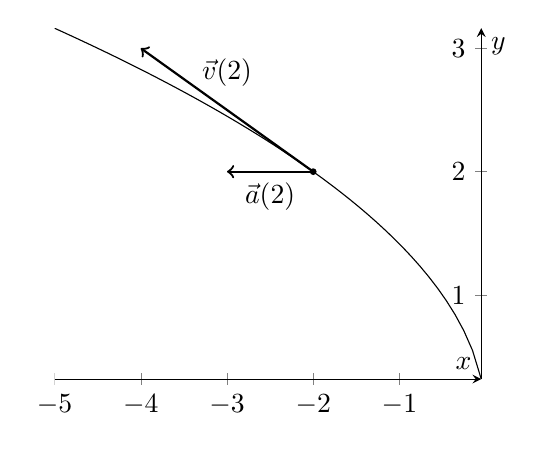
\begin{tikzpicture}
    \begin{axis}[
        axis lines = middle,
        xlabel = \(x\),
        ylabel = {\(y\)},
    ]
    % draw the path
    \addplot[
        color=black,
        samples = 100,
    ]
    {sqrt(-2 * x)}; % function
    % draw the point at t = 2
    \draw[fill=black] (axis cs: -2, 2) circle[radius=1pt];
    % draw the velocity vector at t = 2
    \draw[->, thick] (axis cs: -2, 2) -- (axis cs: -4, 3);
    \node at (axis cs: -3, 2.8) {$\vec v (2)$};
    % draw the acceleration vector at t = 2
    \draw[->, thick] (axis cs: -2, 2) -- (axis cs: -3, 2);
    \node at (axis cs: -2.5, 1.8) {$\vec a (2)$};
    \end{axis}
\end{tikzpicture}

\subsubsection*{5. $\rvec = 3 \cos t \ihat + 2 \sin t \jhat \quad t = \frac \pi 3 $}
\subsubsection*{Solution}
\begin{align*}
    \vcd r t &= \vc v t = \vv{-3\sin t, 2\cos t} \rr \vc v {\frac \pi 3} = \vv{-3(\frac {\sqrt 3} 2), 2(\frac 1 2)} = \vv{-\frac {3\sqrt 3} 2, 1} \\
    \vcdd rt &= \vc a t = \vv{-3\cos t, -2\sin t} \rr  \vc a {\frac \pi 2} = \vv{-3(\frac 1 2), -2(\frac {\sqrt 3} 2)} = \vv{\frac {-3} 2, -\sqrt 3} \\
    \mgv{\vc v t} &= \sqrt{(-3\sin t)^2 + (2\cos t)^2} = \sqrt{9\sin^2 t + 4\cos^2 t} = \sqrt{9(1-\cos^2 t) + 4\cos^2 t} = \sqrt{9 - 5\cos^2 t} \\
\end{align*}
\begin{tikzpicture}
    \begin{axis}[
        axis lines = middle,
        xlabel = \(x\),
        ylabel = {\(y\)},
        xmin = -4, xmax = 4,
        ymin = -4, ymax = 4,
        clip = false
    ]
    % draw the path
    \addplot[
        color=black,
        samples = 100,
        domain = =180:180
    ]
    ({3 * cos(deg(x))}, {2 * sin(deg(x))}); % parametric function
    % draw the point at t = pi/3
    \draw[fill=black] (axis cs: 1.5, sqrt(3)) circle[radius=1pt]);
    % draw the velocity vector at t = pi/3
    \draw[->, thick] (axis cs: 1.5, sqrt(3)) -- (axis cs: ((1.5 - (3*sqrt(3)*0.5)), (sqrt(3) + 1)));
    \node at (axis cs: 1.8, 3) {$\vec v (\frac \pi 3)$};
    % draw the acceleration vector at t = pi/3
    \draw (axis cs: 1.5, sqrt(3)) -- (axis cs: 0, 0);
    \node at (axis cs: 0.6, 1.3) {$\vec a (\frac \pi 3)$};
    \end{axis}
\end{tikzpicture}
\subsubsection*{7. $\rvec = t\ihat + t^2\jhat + 2\khat \quad t = 1$}
\subsection*{Problems 9-13 odd}
        
Find the velocity, acceleration, and speed of a particle with the given position function.

\subsubsection*{9. $\rvec = \langle t^2+ t, t^2 - t, t^3 \rangle $}
\subsubsection*{11. $\rvec = \sqrt 2 t\ihat + e^t\jhat + e^{-t} \khat$}
\subsubsection*{13. $\rvec = e^t(\cos t\ihat + \sin t\jhat + t\khat)$}
\subsection*{Problem 15}

Find the velocity and position vectors of a particle that has the given acceleration and the given initial velocity and position.
\[
    a(t) = 2\ihat + 2t\khat, \quad v(0) = 3\ihat - \jhat, \quad r(0) = \jhat + \khat
\]

\subsection*{Problem 17a}

Find the position vector of a particle that has the given acceleration and the specified initial velocity and position.
\[
    a(t) = 2t\ihat + \sin t\jhat + \cos 2t\khat, \quad v(0) = \ihat, \quad r(0) = \jhat
\]

\subsection*{Problem 23}

A projectile is fired with an initial speed of $200\frac m s$ and angle of elevation $60 \degree$. Find $(a)$ the range of the projectile, $(b)$ the maximum height reached, and $(c)$ the speed at impact.

\subsection*{Problem 26}

A projectile is fired from a tank with initial speed $400 \frac m s$. Find two angles of elevation that can be used to hit a target $3000m$ away.

\subsection*{Problem 27}

A rifle is fired with angle of elevation $36\degree$. What is the initial speed if the maximum height of the bullet is $1600 ft$?

\subsection*{Problem 37 \& 39}

Find the tangential and normal components of the acceleration vector.

\subsubsection*{37. $\rvec = (t^2 + 1)\ihat + t^3\jhat, \quad t \geq 0    $}
\subsubsection*{39. $\rvec = \cos t\ihat + \sin t\jhat + t\khat$}
\subsection*{Problem 41}

Find the tangential and normal components of the acceleration vector at the given point.
\[
    \rvec = \ln t\ihat + (t^2 + 3t)\jhat + 4\sqrt t\khat, \quad (0, 4, 4)
\]


\end{document}
